In this section, we will focus on modeling the airflow around the previously interpolated wing (both the upper and lower parts of the wing).
\subsection{Modelling the airflow}
The subject explains that the airflow is laminar. This means that it can be divided into two parts, and each air molecule moves along curves that do not intersect. Let $h_{min}^{m}$ and $h_{max}^{m}$ be the minimum and maximum height of the airflow, respectively. We assume that the airflow is disturbed by the wing in a vertical interval of $[[3h_{min}; 3h_{max}]]$, otherwise it is rectilinear. Finally, let $y$ be the curve modeling either the extrados or the intrados (by replacing $h_{max}$ with $h_{min}$ of the wing):
\begin{equation}
    \label{eq:equation_part3.1}
    y = f_{\lambda}(x) = (1 - \lambda)f(x) + \lambda \times h_{max} \times 3 \quad \forall \lambda \in [0,1] 
\end{equation}
Using the extrados $x/y$ $(ex, ey)$, the intrados $x/y$ $(ix, iy)$, the function that interpolates the points of the upper part of the wing (fint\_upp), and the function that interpolates the points of the lower part of the wing (fint\_low), we obtain this figure \ref{fig:laminar}, which confirms the laminar nature of the airflow:
\begin{figure}[h]
  \centering
  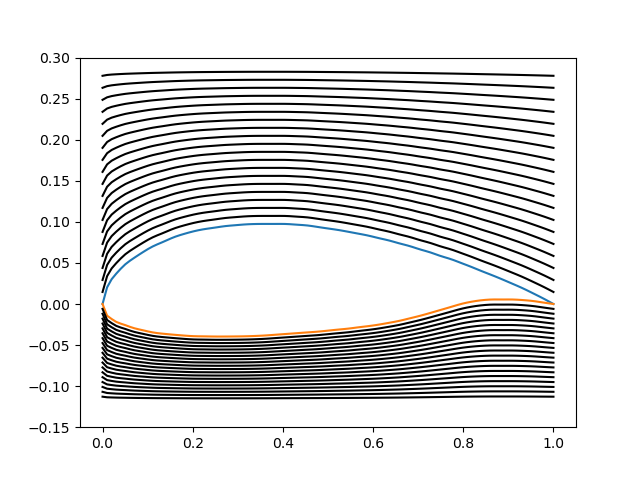
\includegraphics[width=0.45\textwidth]{img/laminar_flow.png}
  \caption{Laminar flow above and below the wing}
  \label{fig:laminar}
\end{figure}

\subsection{Pressure map}

As in the first subsection, we will use functions defined in the previous sections to approach the study of this subsection.
We must plot the function corresponding to the pressure distribution around the wing to have even more information on the aerodynamic profile and thus improve performance and characteristics.\\
We can ultimately come to understand the behavior of the air around the airfoil.\\
Given a laminar airflow, the particles move along independent trajectories.\\
In this sequence, we base ourselves on the distribution of the pressure in the surface of the aerodynamic profile drawn and we save the results.\\
And so does the pressure map obteined shows the informations about the airflow around the airfoil, and shows that the air moves more easily above the wing than below, which leads to a remarkable pressure difference, which in turn creates a lift force that gives the plane the ability to stay aloft?\\
\begin{figure}[h]
  \centering
  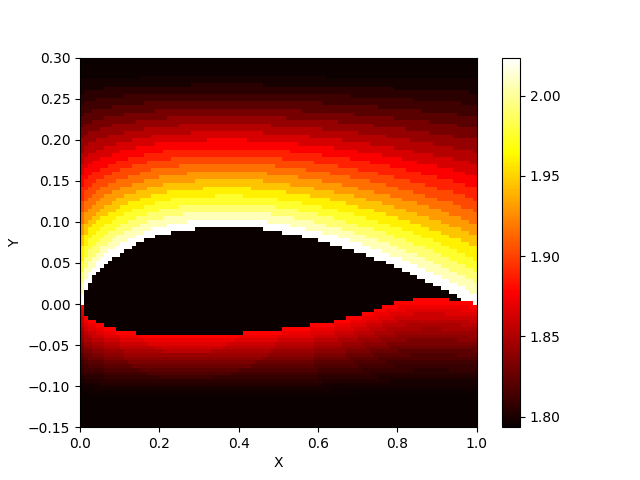
\includegraphics[width=0.45\textwidth]{img/pressure_map.png}
  \caption{Pressure map}
  \label{fig:pressure}
\end{figure}
